


\section{Analysis Results}
The analysis was guided by the previously mentioned research questions. This section will then be organized to answer them in order.

\subsection{Prevalence}

To answer research question (1) in the most broad sense possible, it is necessary to look at how many messages we found that discuss rejuvenation.

The total number of messages collected from the mailing list was 253,548. Also, from the research procedures, we found 603 that were considered as containing code rejuvenation discussion. With this, those 603 messages represent 0.24\% of the total amount. Since this was not an extensive search for those messages, we will consider this, at most, a lower bound.

{\color{red}If we were to trust blindly the selection of threads that was conducted before the manual analysis, assuming every message in every thread selected contained rejuvenation-related discussion, that would be a total of 2639 rejuvenation messages. This represents 1.04\% of the total amount, which we will consider a naive upper bound.

\textbf{Therefore, a rough estimate for how much of the total messages were related to code rejuvenation is between 0.24\% and 1.04\%.}}

Analyzing further, of the 603 selected messages we found the distribution of occurrences present in Figure \ref{fig:msg_year}. Figure \ref{fig:prop_year} indicates what percentage those message occurrences represented of the total number of messages posted in that year. Of those distributions we get an average of 23.2 rejuvenation messages per year and 0.48\% presence per year.

From the manual analysis we determined that the discussions before and after 2011 were fundamentally different in nature. Before 2011 rejuvenation discussion was basically only about compiler support. With the release of C++11, the messages from 2011 onwards are much more like what we expected of code rejuvenation discussion, talking mostly about language standards and features and why to use them or not. This type of discussion relates more to language evolution, as opposed to the compilers available. Not to mention, rejuvenation discussion was much more frequent from 2011 onwards, as is evident in the distributions shown.

Analyzing the same data but limiting the scope to only 2011 onwards, we get an average of 43.2 messages per year, and an average of 0.94\% presence per year.

Moreover, from 2011 onwards the total number of messages collected is 80,043, which is significantly smaller than the whole corpus of messages. However, considering the estimates calculated previously, the number of messages selected manually drops only to 562, which gives us a lower bound of 0.7\% of presence.

\begin{figure}[h]
  \centering
  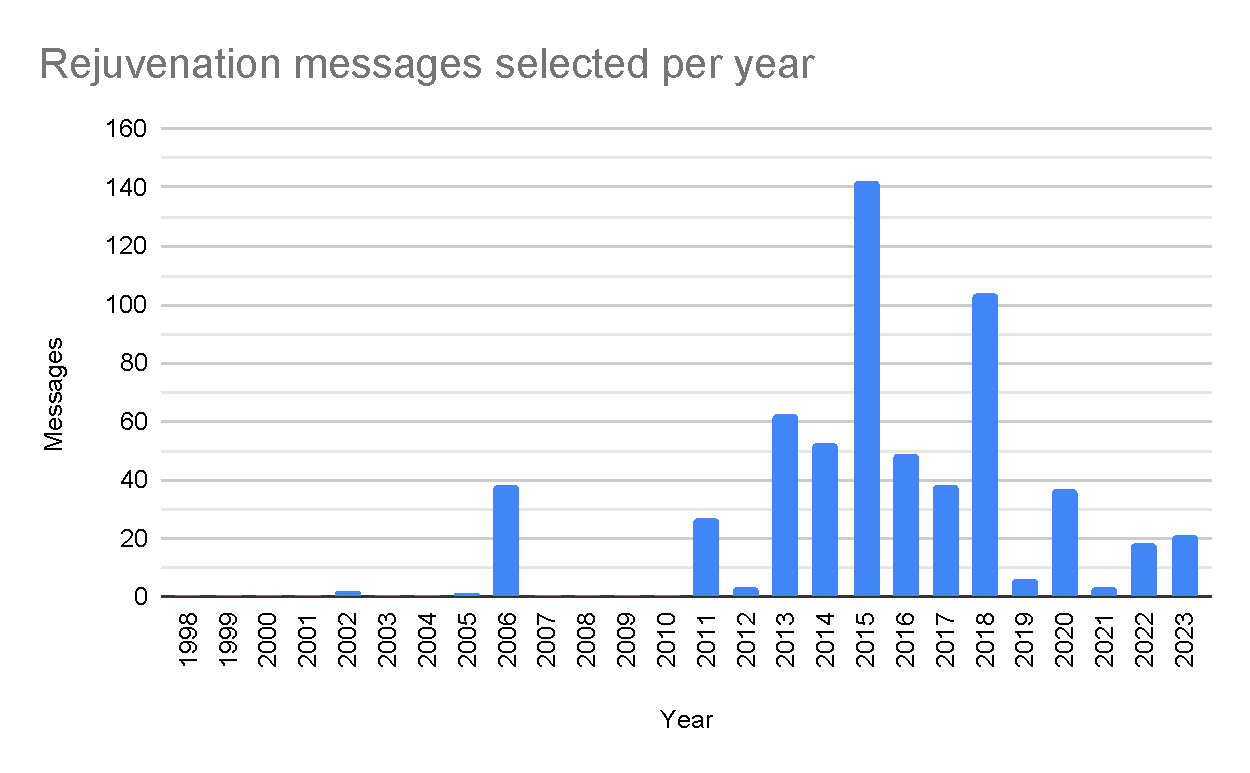
\includegraphics[width=\linewidth]{images/rejuv_msg_per_year.pdf}
  \caption{Distribution of rejuvenation messages found by year}
  \Description{A histogram of how many messages related to source code rejuvenation were found in a given year from 1998 to 2023 in the Boost mailing list.}
  \label{fig:msg_year}
\end{figure}

\begin{figure}[h]
  \centering
  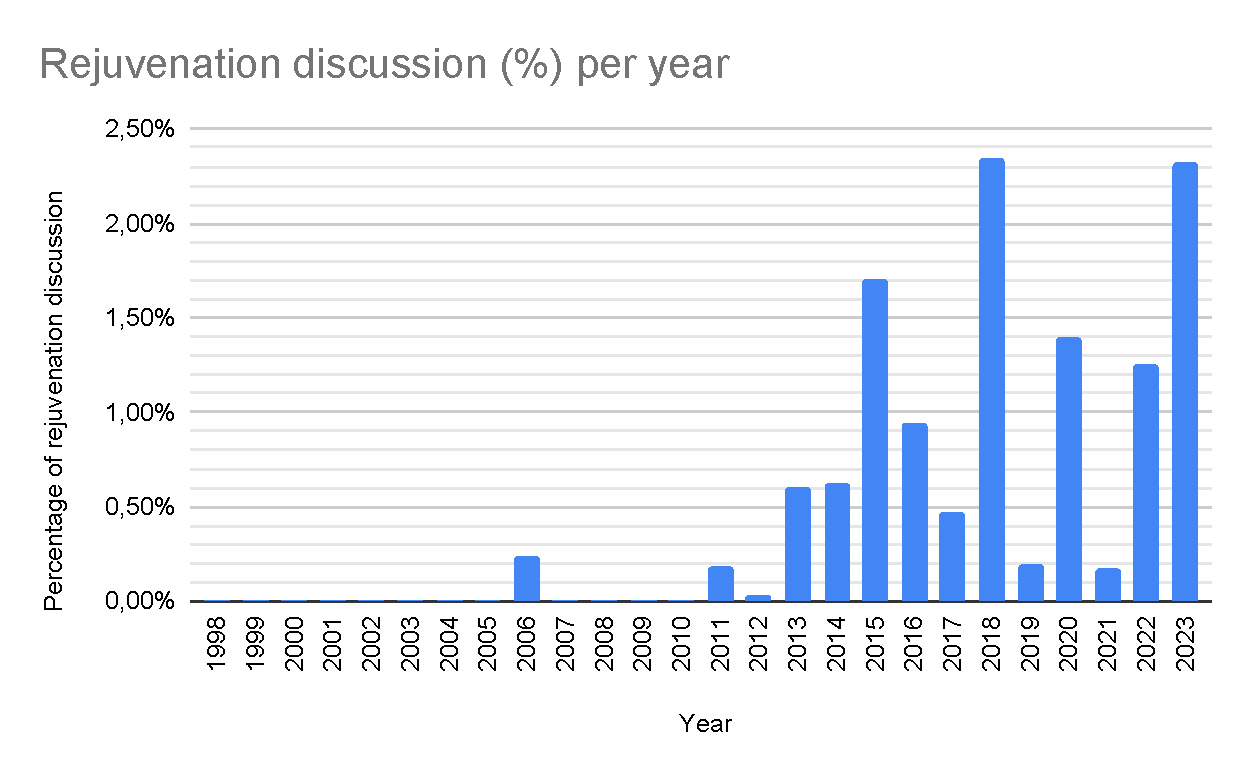
\includegraphics[width=\linewidth]{images/rejuv_proportion_per_year.pdf}
  \caption{Percentage of rejuvenation messages found by year}
  \Description{A histogram of how much of the messages were related to rejuvenation from the total messages posted in a given year from 1998 to 2023 in the Boost mailing list.}
  \label{fig:prop_year}
\end{figure}

{\color{red}The naive upper bound is affected similarly. From 2011 onwards, the number of messages contained in the selected threads is 2532, which now represents 3.16\% of the total amount.

\textbf{Therefore, a rough estimate of code rejuvenation discussion presence from 2011 onwards is in between 0.7\% and 3.16\%.}}

These message distributions, however, pose a contradicting trend. Even though total code rejuvenation-related message numbers declined after 2018, the percentage those numbers represent from the year's total messages have an increasing trend. This can be explained by an overall trend of reduced usage of the Boost mailing list, which was attributed in some messages inside the mailing list to developers moving discussions to GitHub, Slack, and other platforms. This fact also explains the dramatic reduction in the total number of messages collected on the analysis from 2011 onwards.

What this suggests is that \textbf{source code rejuvenation discussion increased in presence even though the mailing list saw decrease in usage.}

Furthermore, analyzing the distribution of messages per year in relation to what was the most recent C++ standard in each year yields an interesting result. In Figures \ref{fig:std_msg_year} and \ref{fig:std_prop_year} we can clearly see peaks in 2015 and 2018. The red color representing C++14 as the most recent standard released and the green color representing C++17, those two peaks seem to align with C++ releases with a 1 year delay. This does not happen equally for C++11 (yellow) nor C++20 (blue) however, although there are peaks in their respective sections.

\begin{figure}[h]
  \centering
  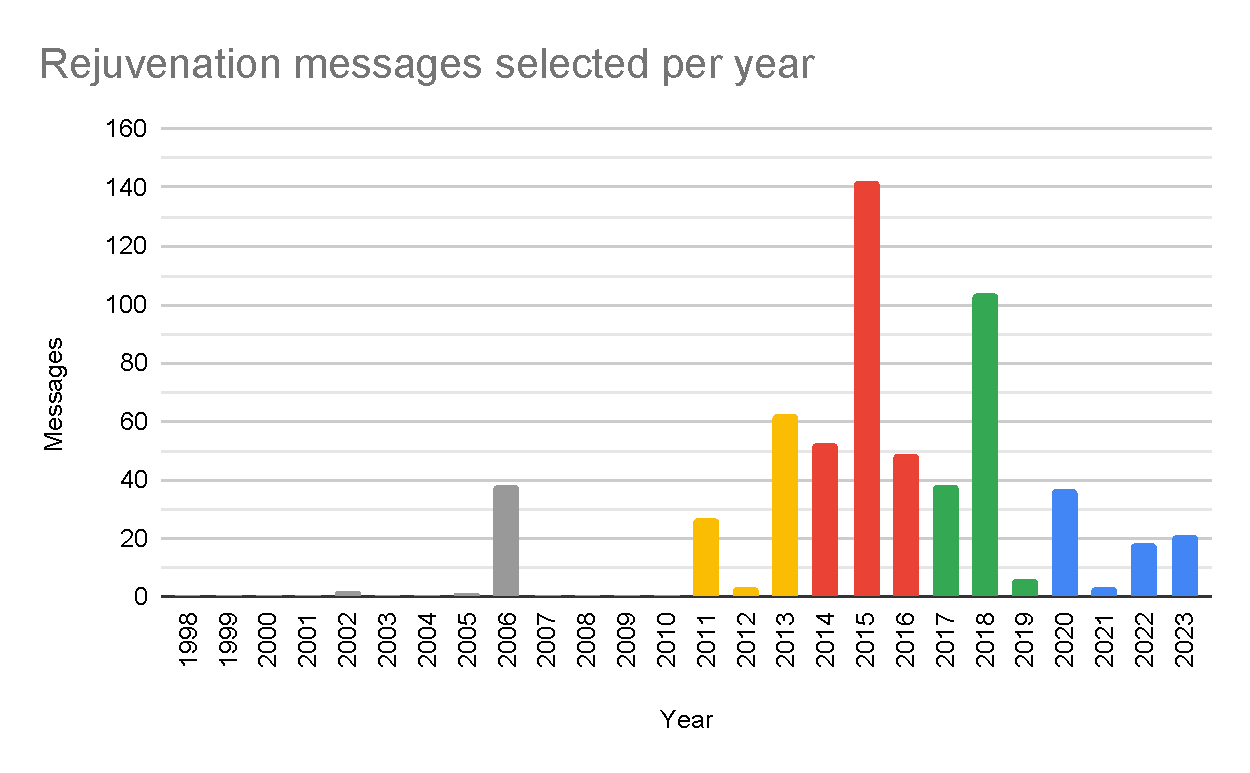
\includegraphics[width=\linewidth]{images/rejuv_msg_per_year_std.pdf}
  \caption{Distribution of rejuvenation messages found by year, colored by most recent C++ standard}
  \Description{A histogram of how many messages related to source code rejuvenation were found in a given year from 1998 to 2023 in the Boost mailing list. The bars are colored according to what C++ standard was the most recent one available at that year.}
  \label{fig:std_msg_year}
\end{figure}

\begin{figure}[h]
  \centering
  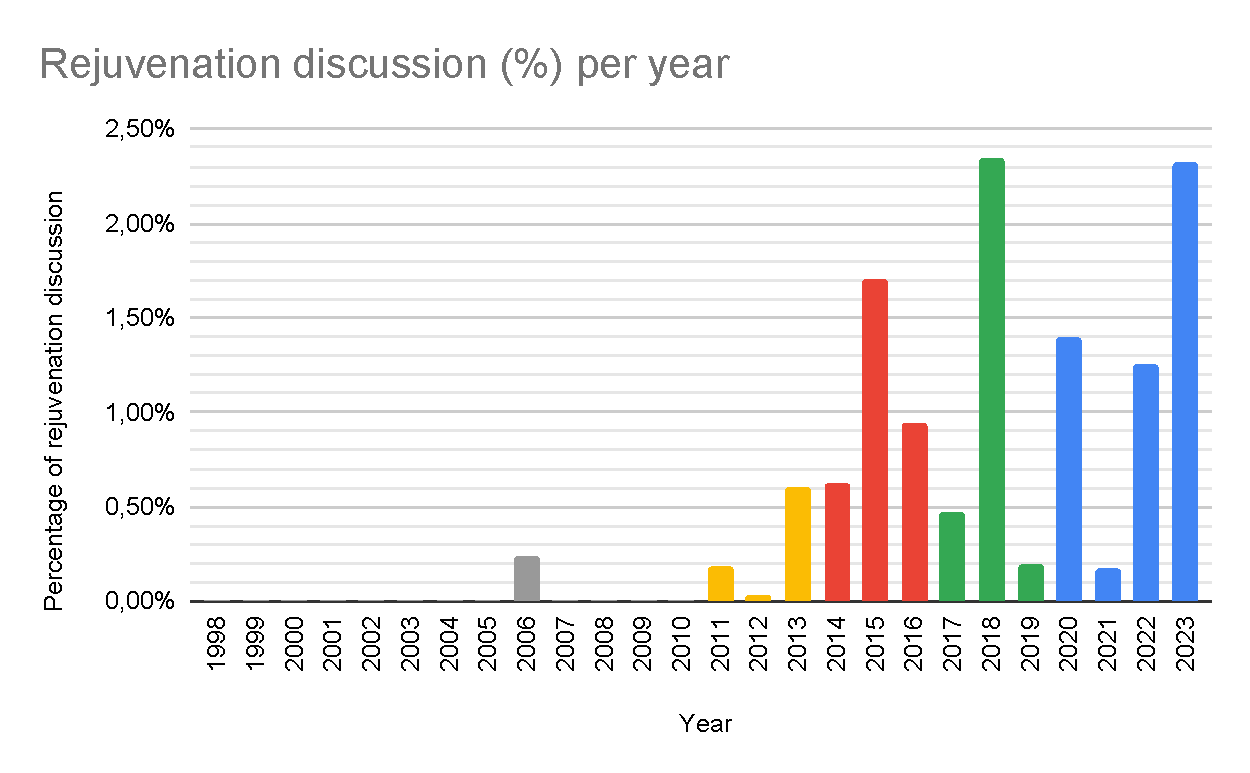
\includegraphics[width=\linewidth]{images/rejuv_proportion_per_year_std.pdf}
  \caption{Percentage of rejuvenation messages found by year, colored by most recent C++ standard}
  \Description{A histogram of how much of the messages were related to rejuvenation from the total messages posted in a given year from 1998 to 2023 in the Boost mailing list. The bars are colored according to what C++ standard was the most recent one available at that year.}
  \label{fig:std_prop_year}
\end{figure}

\textbf{This suggests a correlation between code rejuvenation discussion occurrence and C++ standard releases.} The 1-year delay observed can be explained due to resistance in adhering to new standards as soon as they're released, either due to bugs in the standard or low expected adherence from C++ developers.




\subsection{Topics}

To answer research question (2), a list of topics was derived, as mentioned previously. For every message selected as rejuvenation-relevant, we noted down what topics were mentioned in it. Within the 603 messages analyzed, there were 998 occurrences of topics, which gives an average of 1.7 topics per message. \textbf{This suggests that messages often talked about more than one topic.}

Of the topics themselves, the occurrence distribution is found in Figure \ref{fig:topic_occurr}. \textbf{The two most mentioned topics were C++11 (mentioned in 50.9\% of messages) and C++03 (40.3\%).} This dominance, paired with the knowledge that the vast majority of these analyzed messages occurred after 2013 (as visible in Figure \ref{fig:msg_year}), suggests that \textbf{there were many discussions regarding these C++ standards many years after their releases, while more recent standards were not discussed as much.} In the case of C++03, in most of its occurrences, it had already completed a decade after its release. C++11 also was mentioned a fair amount 5+ years after its release.

\begin{figure}[h]
  \centering
  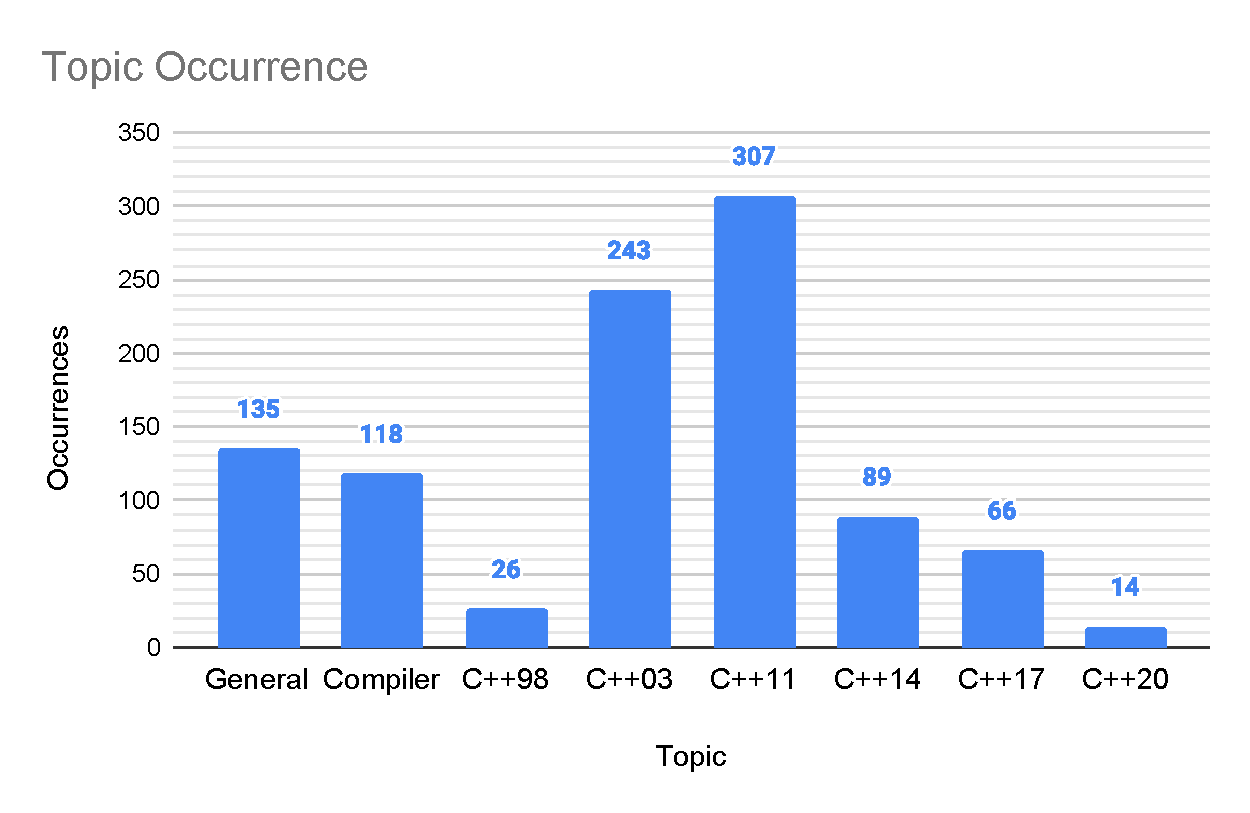
\includegraphics[width=\linewidth]{images/topic_occurrence.pdf}
  \caption{Bar graph of occurrences of topics within rejuvenation discussion}
  \Description{A comparison between the topics listed and tracked, showing how many times each one occurred in the dataset.}
  \label{fig:topic_occurr}
\end{figure}

While analyzing the distribution of each topic by year, we noticed, as shown in Figure \ref{fig:cpp03_11_year}, that, besides being the most popular topics overall, the occurrences of C++03 and C++11 seemed to correlate heavily with one another. In the joint histogram, it is possible to see many similar peaks between the two topics, most notably in 2011, 2015 and 2018.

\begin{figure}[h]
  \centering
  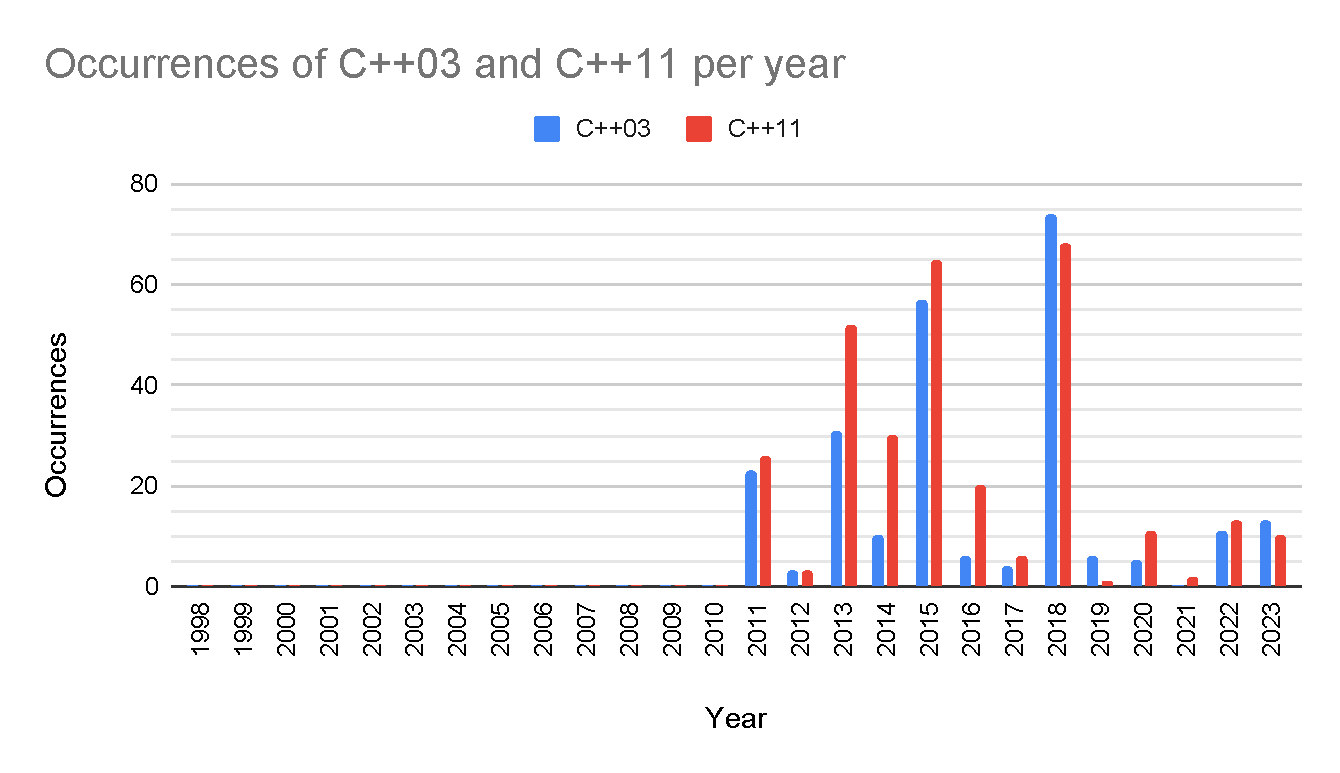
\includegraphics[width=\linewidth]{images/cpp03_11_year.pdf}
  \caption{Distribution of occurrences of C++03 (blue) and C++11 (red) by year}
  \Description{Histogram of occurrences of topics C++03 and C++11 by year. Both distribution's shapes are fairly similar to one another.}
  \label{fig:cpp03_11_year}
\end{figure}

\begin{table*}
\caption{Mutual occurrences between code rejuvenation topics}
  \label{tab:mut_occurr}
\begin{tabular}{@{}lcccccccc@{}}
\toprule
                                    & \multicolumn{1}{l}{General} & \multicolumn{1}{l}{Compilers} & \multicolumn{1}{l}{C++98} & \multicolumn{1}{l}{\textbf{C++03}} & \multicolumn{1}{l}{\textbf{C++11}} & \multicolumn{1}{l}{C++14} & \multicolumn{1}{l}{C++17} & \multicolumn{1}{l}{C++20} \\ \midrule
\multicolumn{1}{l|}{General}        & -                           & 2                             & 0                         & 2                                  & 0                                  & 0                         & 0                         & 0                         \\
\multicolumn{1}{l|}{Compiler}      & 2                           & -                             & 6                         & 26                                 & 33                                 & 7                         & 8                         & 1                         \\
\multicolumn{1}{l|}{C++98}          & 0                           & 6                             & -                         & 14                                 & 18                                 & 8                         & 5                         & 0                         \\
\multicolumn{1}{l|}{\textbf{C++03}} & 2                           & 26                            & 14                        & -                                  & \textbf{188}                       & 29                        & 24                        & 10                        \\
\multicolumn{1}{l|}{\textbf{C++11}} & 0                           & 33                            & 18                        & \textbf{188}                       & -                                  & 72                        & 38                        & 10                        \\
\multicolumn{1}{l|}{C++14}          & 0                           & 7                             & 8                         & 29                                 & 72                                 & -                         & 27                        & 5                         \\
\multicolumn{1}{l|}{C++17}          & 0                           & 8                             & 5                         & 24                                 & 38                                 & 27                        & -                         & 10                        \\
\multicolumn{1}{l|}{C++20}          & 0                           & 1                             & 0                         & 10                                 & 10                                 & 5                         & 10                        & -                         \\ \bottomrule
\end{tabular}
\end{table*}


\begin{table*}
\caption{Percentage of mutual occurrences between code rejuvenation topics}
  \label{tab:mut_occurr_prop}
\begin{tabular}{@{}lcccccccc@{}}
\toprule
                                    & \multicolumn{1}{l}{General} & \multicolumn{1}{l}{Compilers} & \multicolumn{1}{l}{C++98} & \multicolumn{1}{l}{\textbf{C++03}} & \multicolumn{1}{l}{\textbf{C++11}} & \multicolumn{1}{l}{C++14} & \multicolumn{1}{l}{C++17} & \multicolumn{1}{l}{C++20} \\ \midrule
\multicolumn{1}{l|}{General}        & -                           & 1,5\%                         & 0,0\%                     & 1,5\%                              & 0,0\%                              & 0,0\%                     & 0,0\%                     & 0,0\%                     \\
\multicolumn{1}{l|}{Compiler}      & 1,7\%                       & -                             & 5,1\%                     & 22,0\%                             & 28,0\%                             & 5,9\%                     & 6,8\%                     & 0,8\%                     \\
\multicolumn{1}{l|}{C++98}          & 0,0\%                       & 23,1\%                        & -                         & 53,8\%                             & 69,2\%                             & 30,8\%                    & 19,2\%                    & 0,0\%                     \\
\multicolumn{1}{l|}{\textbf{C++03}} & 0,8\%                       & 10,7\%                        & 5,8\%                     & -                                  & \textbf{77,4\%}                    & 11,9\%                    & 9,9\%                     & 4,1\%                     \\
\multicolumn{1}{l|}{\textbf{C++11}} & 0,0\%                       & 10,7\%                        & 5,9\%                     & \textbf{61,2\%}                    & -                                  & 23,5\%                    & 12,4\%                    & 3,3\%                     \\
\multicolumn{1}{l|}{C++14}          & 0,0\%                       & 7,9\%                         & 9,0\%                     & 32,6\%                             & 80,9\%                             & -                         & 30,3\%                    & 5,6\%                     \\
\multicolumn{1}{l|}{C++17}          & 0,0\%                       & 12,1\%                        & 7,6\%                     & 36,4\%                             & 57,6\%                             & 40,9\%                    & -                         & 15,2\%                    \\
\multicolumn{1}{l|}{C++20}          & 0,0\%                       & 7,1\%                         & 0,0\%                     & 71,4\%                             & 71,4\%                             & 35,7\%                    & 71,4\%                    & -                         \\ \bottomrule
\end{tabular}
\end{table*}


\begin{table*}
\caption{Multiplied percentage of mutual occurrences between code rejuvenation topics}
  \label{tab:mut_occurr_mux}
\begin{tabular}{@{}lcccccccc@{}}
\toprule
                                    & \multicolumn{1}{l}{General} & \multicolumn{1}{l}{Compilers} & \multicolumn{1}{l}{C++98} & \multicolumn{1}{l}{\textbf{C++03}} & \multicolumn{1}{l}{\textbf{C++11}} & \multicolumn{1}{l}{C++14} & \multicolumn{1}{l}{C++17} & \multicolumn{1}{l}{C++20} \\ \midrule
\multicolumn{1}{l|}{General}        & -                           & 0,0\%                         & 0,0\%                     & 0,0\%                              & 0,0\%                              & 0,0\%                     & 0,0\%                     & 0,0\%                     \\
\multicolumn{1}{l|}{Compilers}      & 0,0\%                       & -                             & 1,2\%                     & 2,4\%                              & 3,0\%                              & 0,5\%                     & 0,8\%                     & 0,1\%                     \\
\multicolumn{1}{l|}{C++98}          & 0,0\%                       & 1,2\%                         & -                         & 3,1\%                              & 4,1\%                              & 2,8\%                     & 1,5\%                     & 0,0\%                     \\
\multicolumn{1}{l|}{\textbf{C++03}} & 0,0\%                       & 2,4\%                         & 3,1\%                     & -                                  & \textbf{47,4\%}                    & 3,9\%                     & 3,6\%                     & 2,9\%                     \\
\multicolumn{1}{l|}{\textbf{C++11}} & 0,0\%                       & 3,0\%                         & 4,1\%                     & \textbf{47,4\%}                    & -                                  & 19,0\%                    & 7,1\%                     & 2,3\%                     \\
\multicolumn{1}{l|}{C++14}          & 0,0\%                       & 0,5\%                         & 2,8\%                     & 3,9\%                              & 19,0\%                             & -                         & 12,4\%                    & 2,0\%                     \\
\multicolumn{1}{l|}{C++17}          & 0,0\%                       & 0,8\%                         & 1,5\%                     & 3,6\%                              & 7,1\%                              & 12,4\%                    & -                         & 10,8\%                    \\
\multicolumn{1}{l|}{C++20}          & 0,0\%                       & 0,1\%                         & 0,0\%                     & 2,9\%                              & 2,3\%                              & 2,0\%                     & 10,8\%                    & -                         \\ \bottomrule
\end{tabular}
\end{table*}

This could be an indicator for a deeper relation regarding both topics. To analyze this further, we computed all mutual occurrences between every pair of topics into Table \ref{tab:mut_occurr}. From this table it is possible to see that C++03 and C++11 occurred together a total of 188 times. This is also the largest amount of any other pair of topics in the table, the second largest being 72 occurrences between C++11 and C++14.

From Table \ref{tab:mut_occurr}, we computed what the amount of mutual occurrences represented from each topic's total occurrence number. The results of this are present in Table \ref{tab:mut_occurr_prop}. We see that the 188 mutual occurrences represented 77.4\% of C++03's total amount of occurrences. For C++11, it represented 61.2\%.

Table \ref{tab:mut_occurr_prop}, however, has many high-percentage cells, some even higher than the two mentioned. This can be due to two factors: One is that the topic in question was only mentioned when another topic also was, but not vice-versa. Another is that the topic in question simply has very low occurrence amount, therefore a high percentage represents only a few mutual occurrences. In both cases, the high percentage is not present on both sides of the occurrence relation. An example of this is the relation between C++20 and C++11: C++20 occurred 71.4\% alongside C++11, but we see that C++11 occurred only 3.3\% alongside C++20. Seeing as the total amount of mutual occurrences between these is only 10, this does not represent a tight relation between these two, rather, we argue it shows a dependance of one topic onto another, but not the other way around.

For that reason, we decided to multiply both percentage scores from each side of the mutual relations represented in Table \ref{tab:mut_occurr_prop}. By multiplying percentages, the result will only be a high number if both sides of the relation represent a high percentage, and will tend sharply to zero if one percentage is very low, prioritizing larger numbers better than taking the average of them. That result is what we see in Table \ref{tab:mut_occurr_mux}. The highest percentage score is seen between C++03 and C++11, and by a fairly large margin, being more than twice as much as the second highest percentage.

\textbf{These results confirm that C++03 and C++11 occurred together more often than not, being the most mutually occurring - both in total amount and in proportion - of every pair of topics.} This also shows that there were some minor mutual occurring relations between C++11 and C++14, C++14 and C++17, and finally C++17 and C++20.



\subsection{Arguments}

To answer research question (3), we started off by classifying every message with a rejuvenation bias of its own. This represents the overall meaning of the whole message, that may contain arguments of all different sorts and rejuvenation biases. \textbf{Of the 603 messages analyzed, we found that 354 (58.7\%) were in favor of rejuvenation efforts, while 140 (23.2\%) were against rejuvenation efforts and 109 (18.1\%) were ambiguous or neutral towards rejuvenation. This suggests an overall imbalance of presence in favor of rejuvenation in the discussions.} This does not answer the question fully, however, as it would be of interest to look at the arguments used in every message individually.

For that, we used the list of argument categories mentioned previously. This list contained 28 arguments that were separated in groups regarding their rejuvenation bias, as "in favor of rejuvenation", "against rejuvenation" and "ambiguous/neutral". From the manual analysis process we computed the number of occurrences for every argument, and from that how much they were present in the analyzed messages, which is what is presented in Table \ref{tab:argument_list}.

\begin{table*}
\caption{Argument list with rejuvenation bias, occurrence count and presence in analyzed messages}
  \label{tab:argument_list}
\begin{tabular}{@{}lccc@{}}
\multicolumn{1}{c}{\textbf{Argument}}          & \textbf{Rejuvenation Bias} & \textbf{Occurrence count} & \textbf{Presence} \\ \midrule
Against obstruction of new standards           & In favor                   & 35                        & 5,8\%             \\
Considers users of newer standards             & In favor                   & 15                        & 2,5\%             \\
Decentralization                               & In favor                   & 11                        & 1,8\%             \\
\textbf{Deprecation / Discontinuation}         & \textbf{In favor}          & \textbf{167}              & \textbf{27,7\%}   \\
Dissatisfaction with resistance to modernizing & In favor                   & 12                        & 2,0\%             \\
In favor of rejuvenation                       & In favor                   & 112                       & 18,6\%            \\
Invest in C++ innovation                       & In favor                   & 48                        & 8,0\%             \\
Maintenance cost of older standards            & In favor                   & 74                        & 12,3\%            \\
Modularization                                 & In favor                   & 44                        & 7,3\%             \\
Obsolescence argument                          & In favor                   & 19                        & 3,2\%             \\
Optimism with newer standards' adoption        & In favor                   & 18                        & 3,0\%             \\
Recommends updating standards                  & In favor                   & 20                        & 3,3\%             \\
Questions motivation for using older standards & In favor                   & 7                         & 1,2\%             \\
Against deprecation / discontinuation          & Against                    & 53                        & 8,8\%             \\
Against versioning                             & Against                    & 13                        & 2,2\%             \\
Considers users of older standards             & Against                    & 85                        & 14,1\%            \\
Cost of updating to newer standards            & Against                    & 29                        & 4,8\%             \\
In resistance to rejuvenation                  & Against                    & 38                        & 6,3\%             \\
Pessimism with newer standards' adoption       & Against                    & 24                        & 4,0\%             \\
Problem in newer standard                      & Against                    & 3                         & 0,5\%             \\
Unable to rejuvenate                           & Against                    & 9                         & 1,5\%             \\
Considers retrocompatibility                   & Ambiguous / Neutral        & 60                        & 10,0\%            \\
Descriptive                                    & Ambiguous / Neutral        & 70                        & 11,6\%            \\
Interdependence problems                       & Ambiguous / Neutral        & 73                        & 12,1\%            \\
Relevance argument                             & Ambiguous / Neutral        & 49                        & 8,1\%             \\
Questions motivation for using newer standards & Ambiguous / Neutral        & 6                         & 1,0\%             \\
Cynicism with community acceptance             & Ambiguous / Neutral        & 13                        & 2,2\%             \\
Versioning                                     & Ambiguous / Neutral        & 91                        & 15,1\%           
\end{tabular}
\end{table*}

We found that the ten most used argument categories were:

\begin{enumerate}
    \item Deprecation / Discontinuation (present in 27.7\% of messages)
    \item In favor of rejuvenation (18.6\%)
    \item Versioning (15.1\%)
    \item Considers users of older standards (14.1\%)
    \item Maintenance cost of older standards (12.3\%)
    \item Interdependence problems (12.1\%)
    \item Descriptive (11.6\%)
    \item Considers retrocompatibility (10.0\%)
    \item Against deprecation / discontinuation (8.8\%)
    \item Relevance argument (8.1\%)
\end{enumerate}

Of these, (1), (2) and (5) were in favor of rejuvenation, expressing, respectively, arguments towards discontinuation of support to older C++ standards, a general opinion in favor of a proposed rejuvenation effort, and citing the costs of continuing to support older standards. Arguments (3), (6) and (8) were considered ambiguous, expressing respectively that versioning could be applied to resolve a rejuvenation issue, saying there was a problem due to strong dependences over many libraries related to rejuvenation, and considered the effort should keep code compatible with older code. Arguments (7) and (10) were considered conceptually neutral, as they were the act of describing in detail a technical aspect to support your position on the matter, or arguing for the relevance or validity of a previous argument made. Finally, (4) and (9) were against rejuvenation, proposing respectively that developers should consider continuing support for users of older C++ standards, and that they were against discontinuation of these standards.

Not included in the list, but next in presence, were two more arguments in favor of rejuvenation that, along with argument (6), characterized the Boost environment and their unique ambitions and problems. These arguments are "(11) Invest in C++ innovation" (8.0\% presence), that expressed a desire to develop in very modern C++ standards in order to create new libraries and tools that could be incorporated into a future standard, and "(12) Modularization" (7.3\% presence) that expressed a desire to reduce the strong linkage between libraries at Boost in order to better resolve rejuvenation issues.

At Boost, some developers expressed concerns and ambitions regarding reestablishing the previous status of Boost as an organization that contributed majorly to C++'s standardization. That they were, regarding C++98 and C++03, but less so from C++11 onwards, which justified the call for considering this objective as a core priority in the group. Also closely related to Boost, their method of distribution and library usage is largely monolithic in nature, and very interconnected between a large number of libraries, which results in an extensive list of dependencies for a lot of Boost functionalities. This is prone to cause many problems in linkage, compilation and runtime, as different libraries are, at launch, free to be written in any modern C++ standard. Throughout the analyzed messages, we saw many messages around issues that regarded library X's developers proposing moving to a newer C++ standard, but being dissuaded from doing so due to library Y's developers, that closely depended on X, not approving of discontinuing support for older C++ standards.

Moreover, of these results and shown in Figure \ref{fig:arg_occurr}, we observe that 48.7\% of arguments used were in favor of rejuvenation, while ambiguous or neutral arguments represented 30.3\% of the total, and arguments against represented only 21.0\%. \textbf{This shows more than double the occurrence of arguments in favor of rejuvenation than there were of arguments against it.} However, since almost a third of arguments used were not clearly defined as to their rejuvenation bias, the overall distribution still remains unclear. For that, we analyzed this group of arguments in further depth.

\begin{figure}[h]
  \centering
  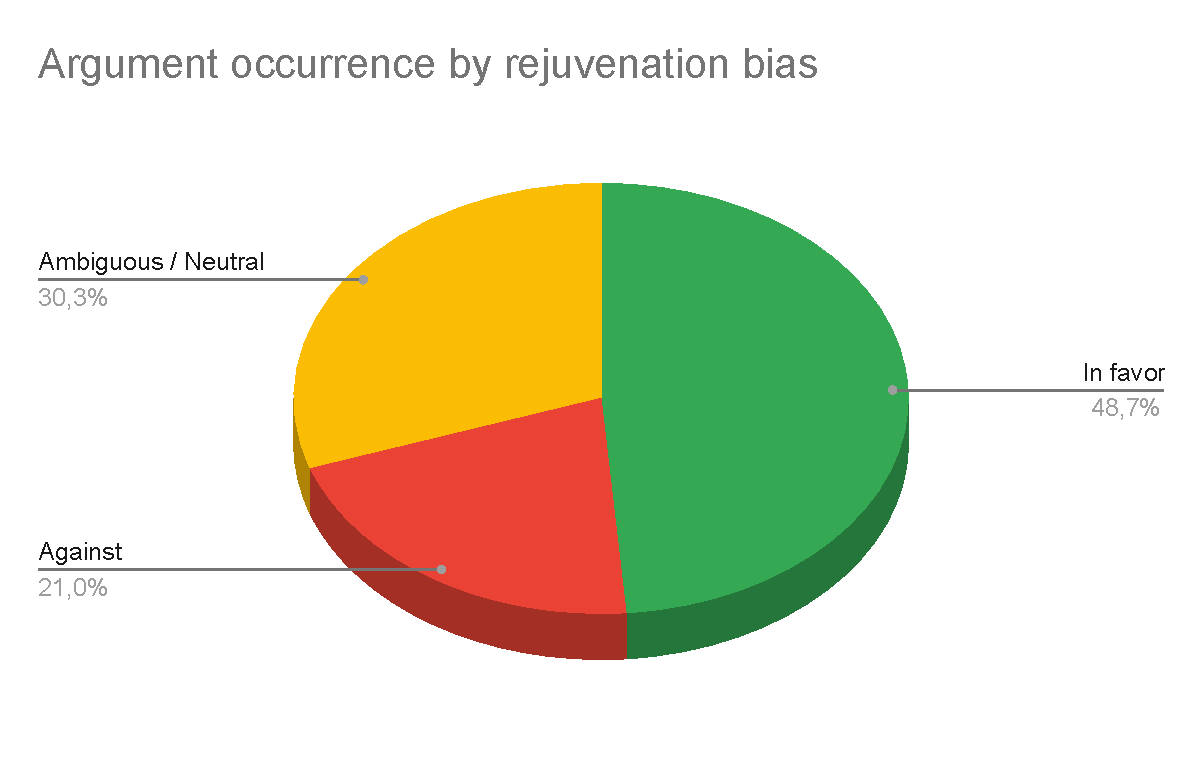
\includegraphics[width=\linewidth]{images/arg_occurr.pdf}
  \caption{Proportion of occurrences of arguments within rejuvenation discussion}
  \Description{A pie graph showing the proportions of occurrences of each group of arguments regarding rejuvenation bias.}
  \label{fig:arg_occurr}
\end{figure}

Of this category of arguments, some were conceptually neutral, like "Descriptive" and "Relevance argument", due to their generalist nature of being discussion tools. That is, both of these express no opinion towards rejuvenation itself, they only explain a related topic in detail or question the relevance and validity of a previous argument in the discussion, and therefore can, in principle, be used equally in both sides of the discussion. However, other arguments in this category were not clearly defined as being predominantly in favor or against rejuvenation.

To determine whether an argument category previously classified as ambiguous had any bias towards rejuvenation, we looked at the classification of the messages where these arguments were found in. Figure \ref{fig:ambg_arg_occurr} shows the total number of occurrences of these arguments, along with sections of how many of these occurred in messages considered in favor of (green), against (red), ambiguous or neutral (yellow) to rejuvenation.

\begin{figure}[h]
  \centering
  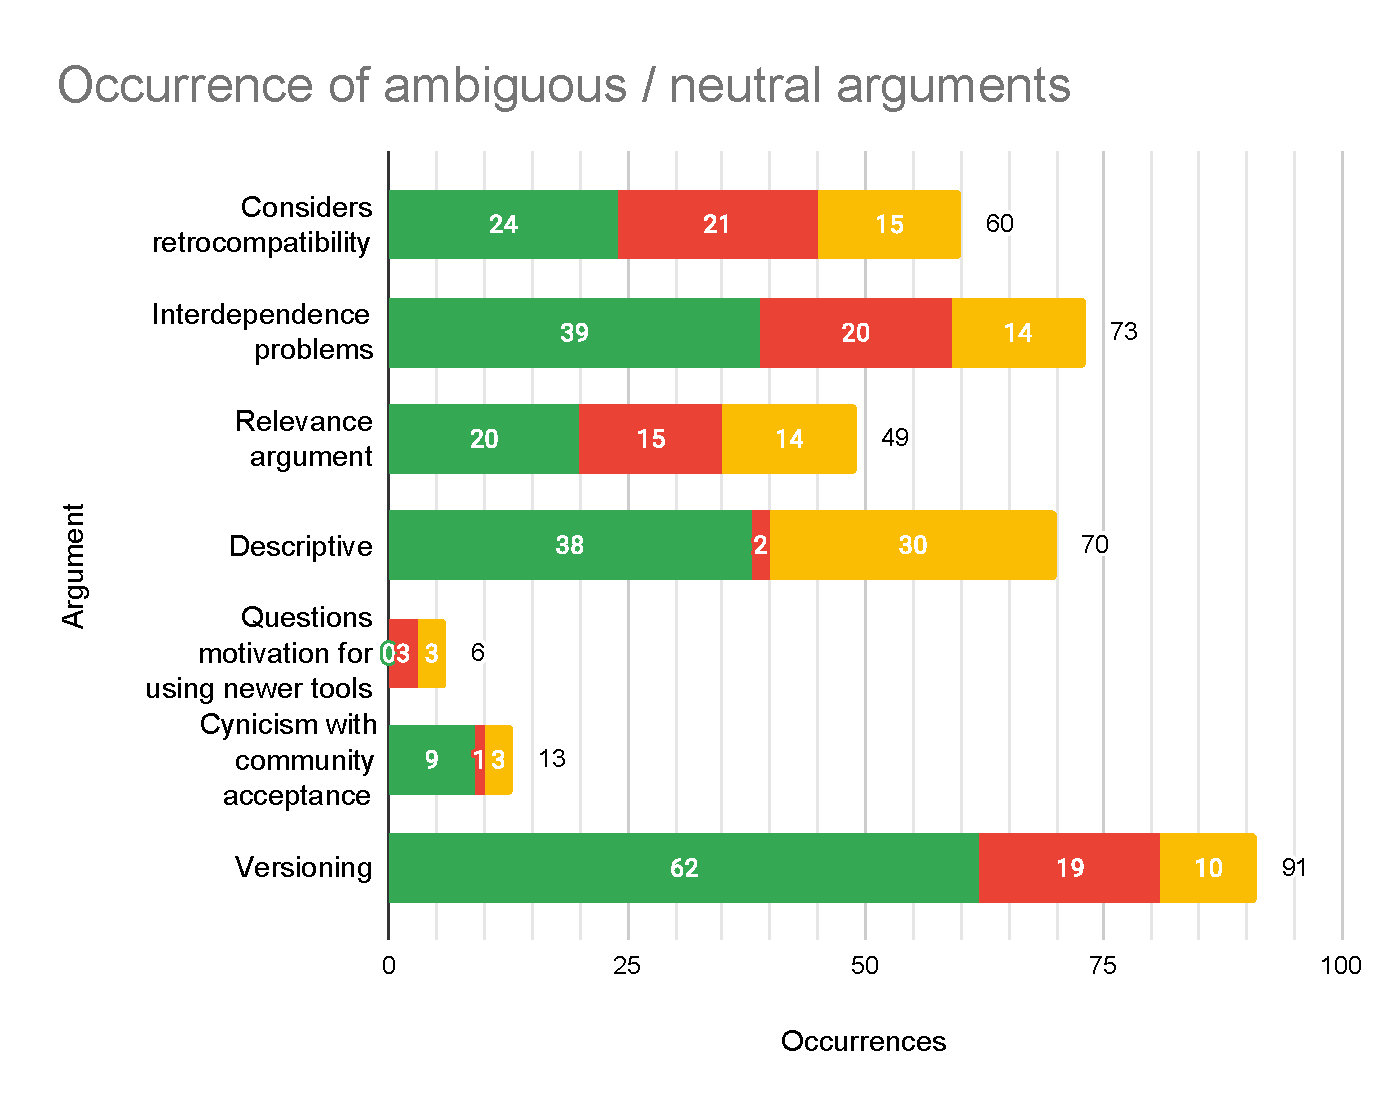
\includegraphics[width=\linewidth]{images/ambg_arg_occurr.pdf}
  \caption{Occurrences of ambiguous or neutral arguments separated by bias of the message they were utilized in}
  \Description{A bar graph showing the occurrences of this category of arguments and the proportions of occurrences in messages of different rejuvenation biases.}
  \label{fig:ambg_arg_occurr}
\end{figure}

From this analysis, we found that arguments such as "Versioning", "Interdependence problems" and "Cynicism with community acceptance" were proportionally more employed in messages classified as in favor of rejuvenation, ranging from 53.4\% to 69.2\% of usage. In contrast, "Questioning motivation for using newer standards" seemed to be mostly used to argue against rejuvenation. Addittionally, "Considering retrocompatibility" was found to be used rather evenly by both sides, with the ambiguous use also being fairly present (25\% of occurrences). "Relevance argument" saw similar usage as the previous ambiguous argument. "Descriptive" was used often by messages in favor of rejuvenation (54.3\%), but almost just as often in ambiguous or neutral messages (42.9\%), which keeps it in an ambiguous or neutral classification.

\textbf{Overall, most uses of "Ambiguous / Neutral" arguments were in messages classified as in favor of rejuvenation. This solidifies the suggested positive bias towards rejuvenation in the arguments found in these discussions.}
